\documentclass[12pt,a4paper]{article}
\usepackage[utf8]{inputenc}
\usepackage[english,russian]{babel}
\usepackage{indentfirst}
\usepackage{misccorr}
\usepackage{graphicx}
\usepackage{amssymb}
\usepackage{amsmath}
\usepackage{wrapfig}

\begin{document}

\begin{center}
    \large
    Работа 2.4.1
    
    Сибгатуллин Булат, Б01-007
    
    \vspace{0.5cm}
    \textbf{Определение теплоты испарения жидкости}

\end{center}

\vspace{0.5cm}
\textbf{Цель работы:} 1) измерение давления насыщенного пара жидкости при рпазной температуре; 2) вычисление по полученным данным теплоты испарения с помощью уравнения Клапейрона-Клазиуса.

\vspace{0.5cm}
\textbf{В работе используются:} термостат; герметический сосуд, заполненный исследуемой жидкостью; отсчетный микроскоп.

\vspace{0.5cm}
Испарением называется переход вещества из жидкого в газообразное состояние. При испарении молекулы вылетают из жидкости, образуя на ней пар, также они должны преодолеть силы молекулярного сцепления и совершить работу пртоив внешнего давления. Поэтому  только молекулы, обладающие достаточной кинетической энергией способны вылететь из жидкости, следовательно, чтобы испарение проходило без изменения температуры, к жидкости нужно подводить тепло. 

В нашей работе для определения теплоты применен метод основанный на формуле Клапейрона-Клаузиуса:

\begin{equation}\label{Klapeiron-Klausius}
\frac{dP}{dT} = \frac{L}{T (V_1 - V_2)}.
\end{equation}

Здесь \textit{P} - давление насыщенного пара жидкости при температуре \textit{T}, \textit{T} - абсолютная температура жидкости и пара, \textit{L} - теплота испарения жидкости, $V_2$ - объём пара, $V_1$ - объём жидкости. Величины \textit{L}, $V_1$ и $V_2$ относятся к одному и тому же количеству вещества, в нашем случае к одному молю.

В нашем приборе измерения производятся при давлениях ниже атмосферного. В этом случае задача существенно успрощается, так как $V_1$ не превосходит $0,5\%$ от $V_2$. При нашей точности опытов величиной $V_1$ можнопренебречь. За \textit{V} обозначим $V_2$, он будет связан с давлением и температурой уравнением Вандер-Ваальса:

\begin{equation}\label{Vander-Vaals}
\Big(P + \frac{a}{V^2}\Big)(V - b) = RT
\end{equation}

В уравнении Вандер-Ваальса величиной по сравнению \textit{b} следует пренебречь. Пренебрежение членом $a/V^2$ по сравнению с \textit{P} вночит ошибку менее $3\%$. При давлении ниже атмосферного ошибки становятся еще меньше, поэтому уравнение Вандер-Ваальма мало отличается от уравнения Клапейрона:

\begin{equation}\label{Klapeiron}
V = \frac{RT}{P}
\end{equation}

Подставляя (\ref{Klapeiron-Klausius}) в (\ref{Klapeiron}), пренебрегая $V_1$ и разрешая уравнение относительно \textit{L}, найдем

\begin{equation}\label{3to1}
L = \frac{RT^2}{P} \frac{dP}{dT} = -R \frac{d(\ln P)}{d(1/T)}
\end{equation}

\begin{wrapfigure}{r}{0.2\textwidth}

\includegraphics[width=0.3\textwidth]{Screenshot_1.png}
\label{ris:image}
\end{wrapfigure}

\textbf{Экспериментальная установка.} Схема установки изображена на рисунке 1. Роль термостата играет наполненный водой резервуар 1. Его нагревание производится спиралью 2, а охлаждение при помощи змеевика 3, через который проходит трубопроводная вода. Вода в термостате перемешивается воздухом, поступающим через трубку 4. Температура воды измеряется термометром 5. в термостат погруже запаянный прибор 6 с исследуемой жидкостью. Давление насыщенного пара определеяется по ртутному манометру. Отсчет показаний манометра производится с помощью микроскопа.

На рисунке 2 приведена более полная схема такой же установки, но с использованием современного термостата. Она включает в себя термостат А, экспериментальный прибор В и отсчетный микроскоп С.

Экспериментальный прибор В представляет собой емкость 12 заполненную водой, в которую погружён запаянный прибор 13 с исследуемой жидкостью 14 (над жидкостью находиться только её насыщенный пар). Давление пара определяется по ртутному манометру 15, соединенному с емкостью 13. Численная величина давления измеряется по разности показаний отчетного микроскопа 16, его показани снимаются по шкале 17.

\begin{figure}[h!]
\centering
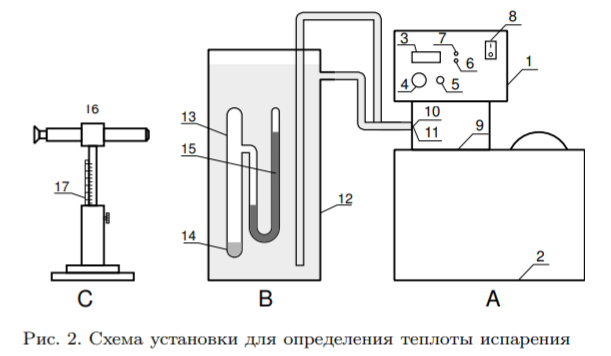
\includegraphics[scale=0.8]{Screenshot_2.png}
\label{fig:Image1}
\end{figure}

\vspace{0.5cm}

\textbf{1.} Проведем измерения и запишем их результаты в таблицы. Первая будет содержать в себе данные температуры и давления при повышении температуры, вторая при понижении. Причем давлении в Паскалях получим из давлени в миллиметрах ртутного столба по формуле:

\[P_{\textit{Па}} = P_{\textit{мм.рт.ст}} * 133,32\]

\begin{tabular}{|c|c|c|c|c|c|c|c|}
\hline 
P, мм.рт.ст. & 35,8 & 37,8 & 41,6 & 43,5 & 46,0 & 49,6 & 52,8 \\ 
\hline 
P, Па & 4772,9 & 5039,6 & 5546,2 & 5799,5 & 6132,8 & 6612,8 & 7039,4 \\ 
\hline 
T, К & 293,5 & 294,7 & 295,7 & 296,5 & 297,5 & 298,9 & 299,5 \\ 
\hline
\hline 
P, мм.рт.ст. & 56,5 & 59,9 & 63,6 & 67,9 & 71 & 76 & 81,1 \\ 
\hline 
P, Па & 7532,7 & 77986,0 & 8479,3 & 9052,6 & 9465,9 & 10132,5 & 10812,5 \\ 
\hline 
T, К &  300,5 & 301,5 & 302,5 & 303,5 & 304,5 & 305,5 & 306,7 \\ 
\hline 
\end{tabular}

\vspace{0.5cm}

\begin{tabular}{|c|c|c|c|c|c|c|c|}
\hline 
P, мм.рт.ст. & 80.0 & 75,8 & 69,9 & 65,8 & 62,0 & 58,9 & 51,4 \\ 
\hline 
P, Па & 10665,8 & 10105,8 & 9319,2 & 8772,6 & 8265,9 & 7852,7 & 6852,8 \\ 
\hline 
T, К & 306,5 & 305,3 & 304,1 & 303,1 & 302,1 & 301,1 & 298,9 \\ 
\hline 
\hline
P, мм.рт.ст. & 48,3 & 46,0 & 42,4 & 39,9 & 37,6 & 35,1 & 32,7 \\ 
\hline 
P, Па & 6439,5 & 6132,8 & 5652,9 & 5319,6 & 5020,0 & 4679,6 & 4259,6 \\ 
\hline 
T, К & 298,1 & 297,1 & 296,1 & 295,1 & 294,1 & 293,1 & 292,1 \\ 
\hline 
\end{tabular} 

\vspace{0.5cm}

Построим графики используя метод наименьших квадратов, в итоге будет получена линейная зависимость вида $y = a + bx$. Так как вычисления занимают много места, они были вынесены в отдельный файл с названием вычисления. Здесь я запишу только итоговые результаты.

1. Для зависимости $P$ от $T$:

$b_1$ = 449,08

$a_1$ = -127251,73

$\sigma_{b_1} = 8,08$

$\sigma_{a_1} = 34,81$

2. Для зависимости \textit{ln(P)} от \textit{1/T}:

$b_2$ = -5613,90

$a_2$ = 27,60

$\sigma_{b_2} = 71,56$ 

$\sigma_{a_2} = 0,00345$

\vspace{0.5cm}

Погрешности измерений определяются их техническими характеристиками:

\[\sigma_T = 0,1 \textit{К} \quad \sigma_P = 13,3 \textit{Па}\]

\[\varepsilon_{T\textit{ср}} = 0,03\% \quad \varepsilon_{Pmax} = 0,3\%\]

Определить погрешности логарифма давления можно по формуле:

\[\sigma_{ln(P)} = \frac{1}{P}\sigma_P\]

\[\sigma_{ln(P)max} = 0,3 \quad \varepsilon_{ln(P)max} = 0,3\%\]

\vspace{0.5cm}

Погрешность температуры в минус превой степени определяется так:

\[\frac{\sigma_{1/T}}{1/T} = \sqrt{\frac{\sigma_T^2}{T^2}}\]

\[\varepsilon_{1/T} = \epsilon_T = 0,3\%\]
\vspace{0.5cm}

\begin{figure}[h!]
\centering
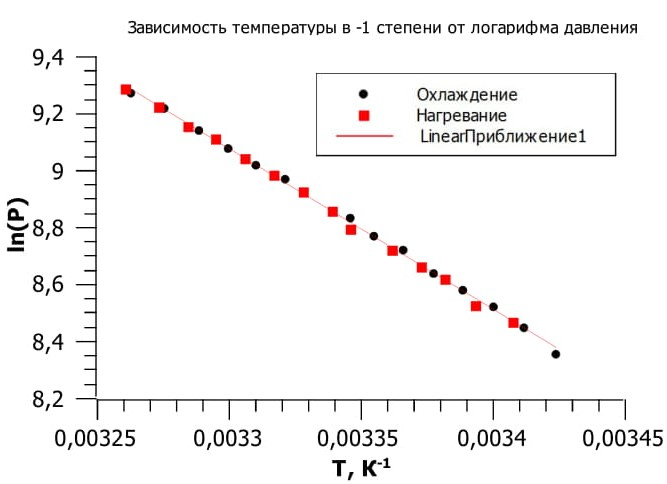
\includegraphics[scale=0.55] {ln(P)-1.jpg}
\label{fig:Image1}
\end{figure}

\vspace{0.5cm}

\begin{figure}[h!]
\centering
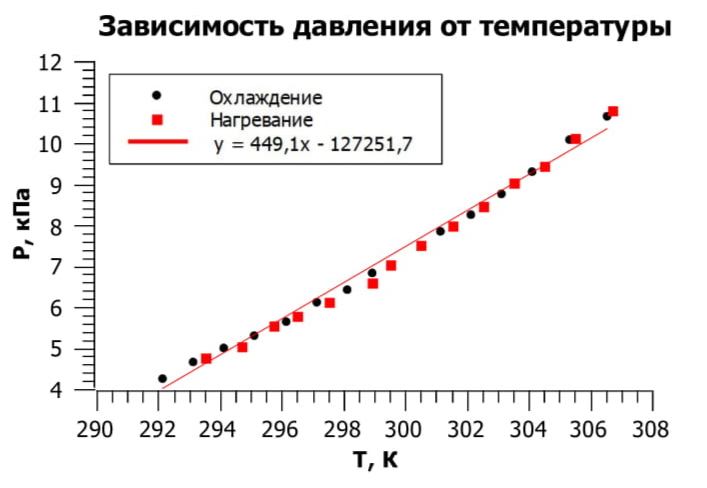
\includegraphics[scale=0.8]{P_V-1.png}
\label{fig:Image1}
\end{figure}
\vspace{0,5cm}

В первом графике L зависит от температуры и давления по формуле (\ref{3to1}), поэтому я возьму среднее значение $\frac{RT^2}{P}$ (оно посчитано в документе с названием вычисления-2.4.1, я перенес их туда, так как они заменяли достаточно много места), а $\frac{dP}{dT}$ возьму как коэффициент $b_1$.

\[L = <\frac{RT^2}{P}> \cdot \frac{dP}{dT} = \frac{R<T^2>}{<P>} \cdot b_1 = 102,51 \cdot 449,08 = 46032,98 \: \textit{Дж}/ \textit{моль}\]

\[\sigma_L = L \sqrt{\Big( \frac{\sigma_{b_1}}{b_1}\Big)^2 + \Big( \frac{\sigma_T }{T}\Big)^2 + \Big( \frac{\sigma_P}{P}\Big)^2} = L\sqrt{\varepsilon_{b_1}^2 + \varepsilon_{T\textit{ср}}^2 + \varepsilon_{P\textit{max}}^2}\]

\[\sigma_L = 46031,98 \cdot \sqrt{0,0179^2+0,003^2 + 0,0003^2} = 837,78 \: \textit{Дж}/ \textit{моль}\]

\vspace{0.5cm}

Во втором графике L находится по формуле (\ref{3to1}):

\[L = -R\frac{d(lnP)}{d(1/T)} = -R \cdot b_2 = 8,31 \cdot 5613,90 = 46651,51 \: \textit{Дж}/ \textit{моль}\]

\[\sigma_L = L \sqrt{\Big( \frac{\sigma_{b_2}}{b_2}\Big)^2 + \Big( \frac{\sigma_{1/T} }{1/T}\Big)^2 + \Big( \frac{\sigma_{lnP}}{lnP}\Big)^2} = L\sqrt{\varepsilon_{b_2}^2 + \varepsilon_{1/T}^2 + \varepsilon_{lnP\textit{max}}^2}\]

\[\sigma_L = 46651,51 \cdot \sqrt{0,0127^2+0,003^2 + 0,0003^2} = 608,94 \: \textit{Дж}/ \textit{моль}\]

\vspace{0.5cm}

\textbf{Вывод.} Значение теплоты измерения в обоих графиках оказалось равным в пределах погрешности:

\[L_1 = 46032,98 \pm 837,78 \: \textit{Дж}/ \textit{моль}, \quad L_2 = 46651,51 \pm 608,94 \: \textit{Дж}/ \textit{моль}\]

Табличные значения для спирта показывают 40000 \textit{Дж}/\textit{моль}, что не совпадает с нашими данными. Этому может быть несколько обьяснений, в нашем опыте используется не чистый спирт, а смесь спирта с другой жидкостью и что наша температура отличается от той, для которой написаны табличные значения.

\vspace{0.5cm}

\textbf{1.} Табличные значения для спирта показывают 40000 \textit{Дж}/\textit{моль}, что не совпадает с нашими данными. Полученные мной данные отличаются от табличных на 15% в большую сторону.

\vspace{0.5cm}

\textbf{2.} Теплота испарения с увеличением температуры должна уменьшаться, так как кинетическая энергия молекул увеличивается, и им нужно дать меньше энергии, чтобы они покинули жидкую среду.

\end{document}